\chapter{สถานที่ปฏิบัติงาน}
บริษัท วงใน มีเดีย จำกัด (สำนักงานใหญ่) ตั้งอยู่ที่อาคารทีวัน ชั้น 26, 27 โดยสามารถเดินทางได้ด้วยรถไฟฟ้า BTS มาที่สถานีทองหล่อ จากนั้นสามารถเดินเข้ามาในอาคารด้วยทางเชื่อมจากสถานีทองหล่อได้ทันที โดยจะได้ปฏิบัติงานบริเวณชั้นที่ 26 เป็นส่วนใหญ่ ในชั้นนี้จะประกอบไปด้วยห้องทำงานแบบเปิดโล่ง ไม่มีฉากกั้น พนักงานแต่ละคนสามารถเดินไปมาหากันได้ มีห้องน้ำ ห้องครัว ห้องโถง และมีอาหารว่างและเครื่องดื่มให้รับประทานตลอดเวลา

\begin{figure}[!h]
	\centering
	\subfigure[บริเวณห้องที่ปฏิบัติงาน]{
		\label{Fig:workspace:desk1}
		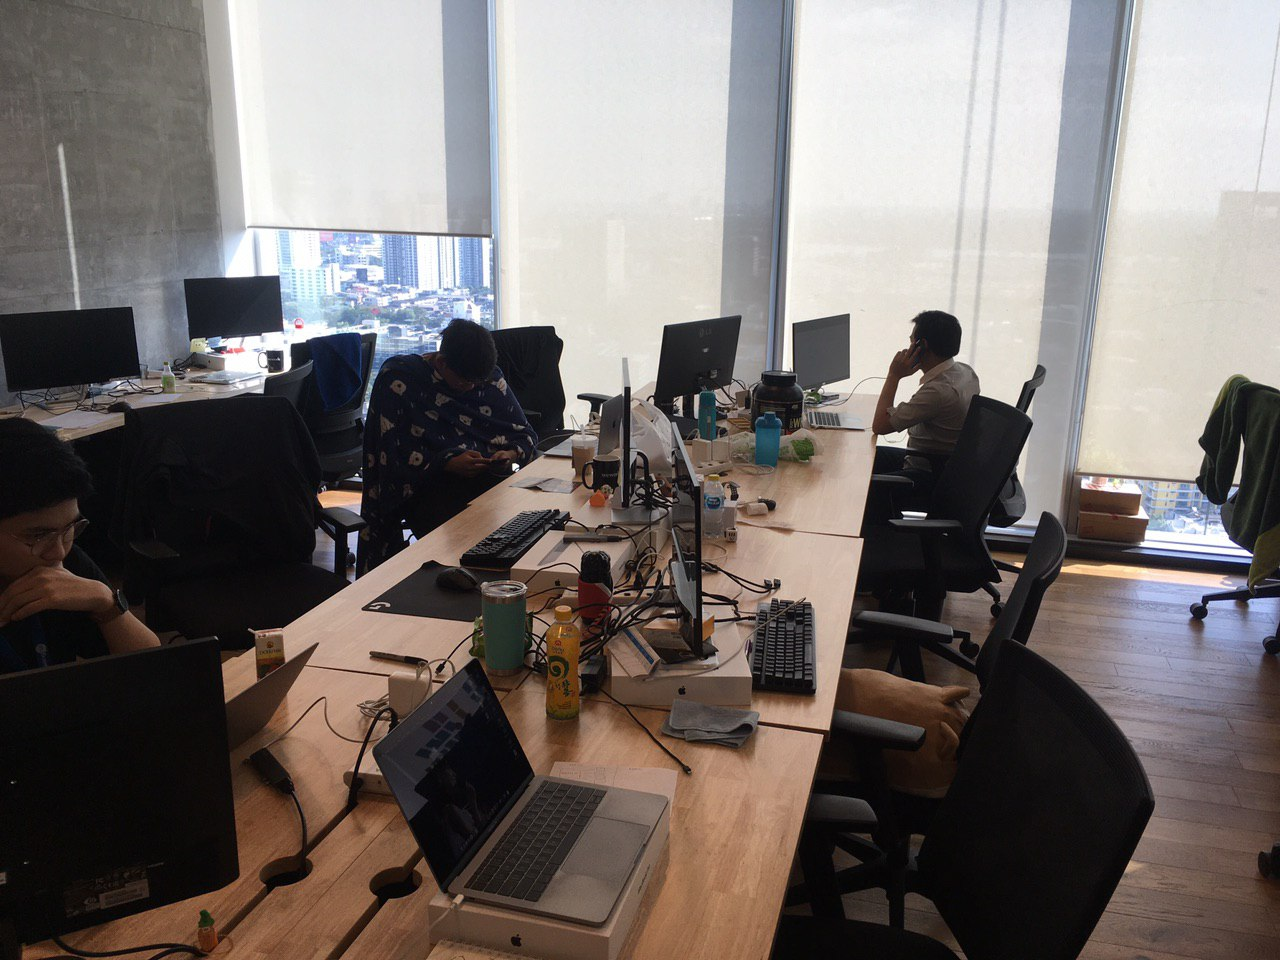
\includegraphics[width=0.47\textwidth]{desk1}  
	}
	\subfigure[บริเวณโต๊ะทำงาน]{
		\label{Fig:workspace:desk2}
		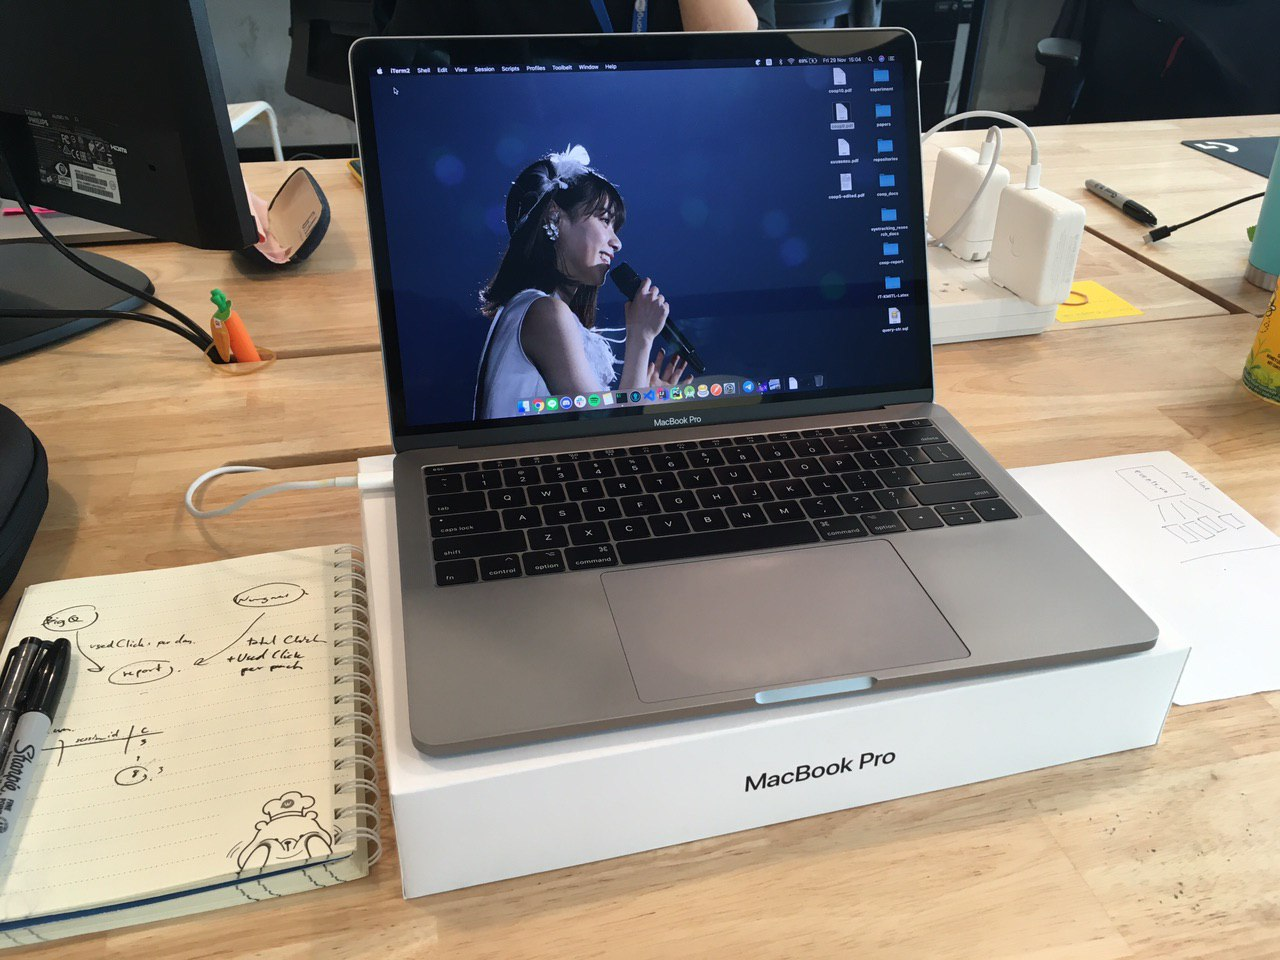
\includegraphics[width=0.47\textwidth]{desk2}  
	}
	\subfigure[บริเวณห้องครัว]{
		\label{Fig:workspace:pantry}
		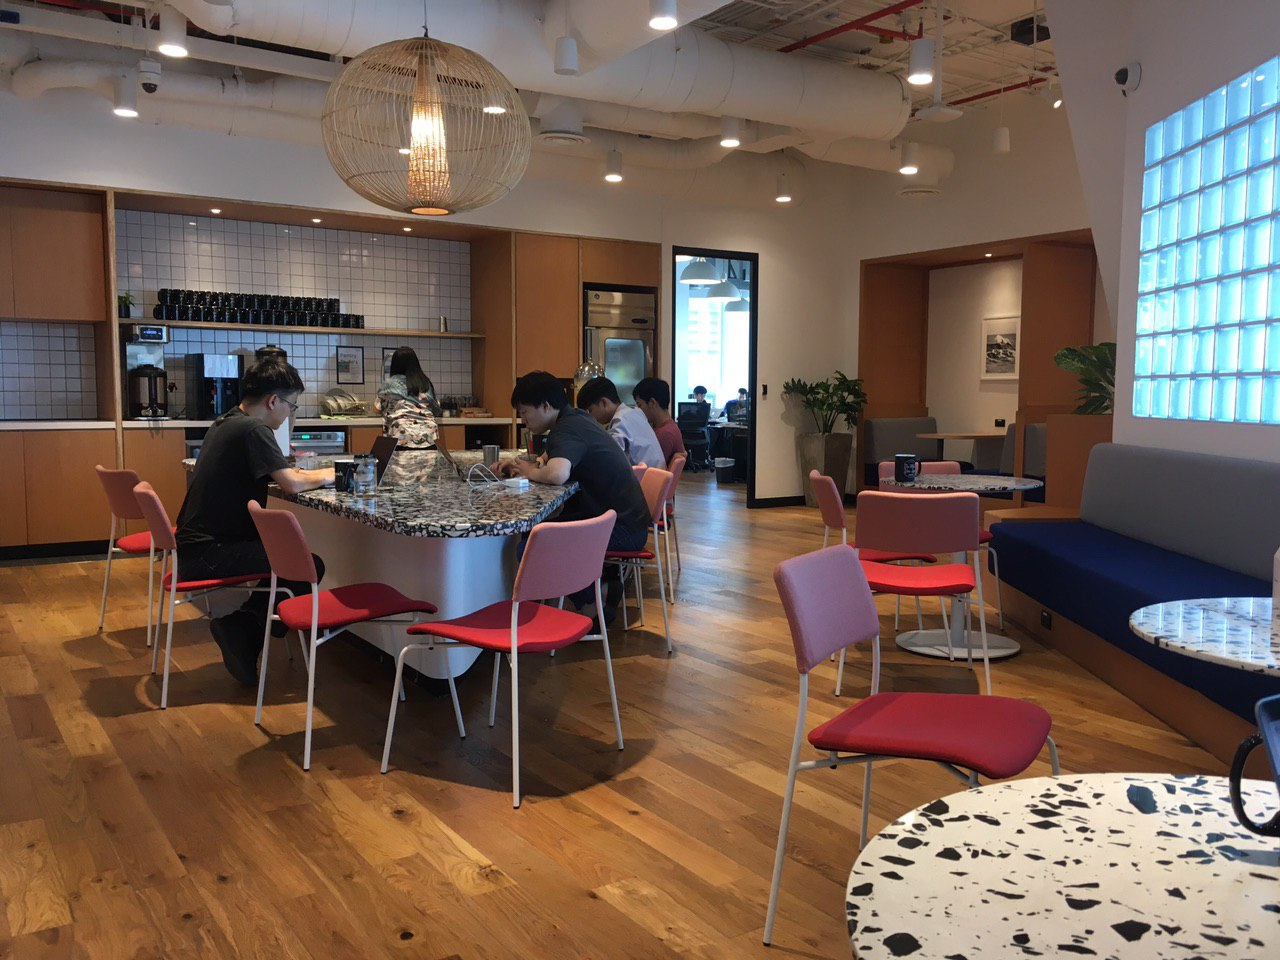
\includegraphics[width=0.6\textwidth]{pantry}  
	}
	\subfigure[ตู้เย็น]{
		\label{Fig:workspace:fridge}
		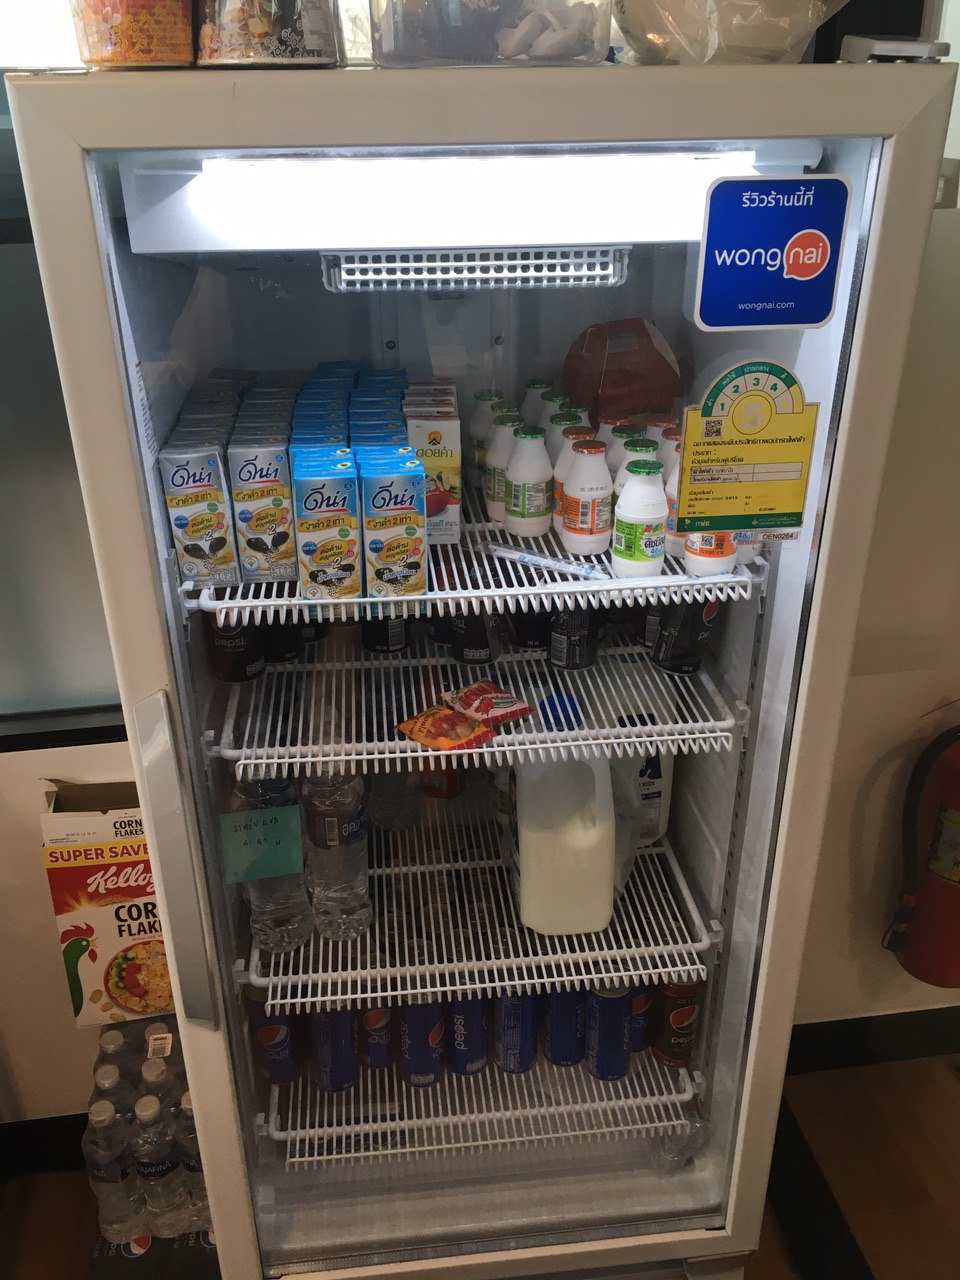
\includegraphics[width=0.34\textwidth]{fridge}  
	}
	\caption{สถานที่ปฏิบัติงาน}
	\label{Fig:workspace}
\end{figure}

\chapter{กิจกรรมระหว่างปฏิบัติงาน}
ในระหว่างการปฏิบัติงาน จะมีกิจกรรมต่าง ๆ อยู่ตลอดเวลา มีทั้งกิจกรรมเพื่อการเรียนรู้และกิจกรรมเพื่อความสนุกสนานและการผ่อนคลาย เช่น 
งานเลี้ยงรับประทานอาหารที่จัดขึ้นทุก ๆ เดือน, กิจกรรม WeShare ซึ่งเป็นกิจกรรมที่จะนำวิทยากรมาบรรยายเรื่องต่าง ๆ ในวันศุกร์, งาน Town Hall ซึ่ง เป็นงานจัดขึ้นทุก ๆ ไตรมาส เพื่อเป็นการรายงานสิ่งที่เกิดขึ้น, ผลงานต่าง ๆ ในไตรมาสนั้นและเป้าหมายในไตรมาสถัดไป และอื่น ๆ อีกมากมาย

\begin{figure}[!h]
	\centering
	\subfigure[งานเลี้ยงรับประทานอาหาร]{
		\label{Fig:even1:eat}
		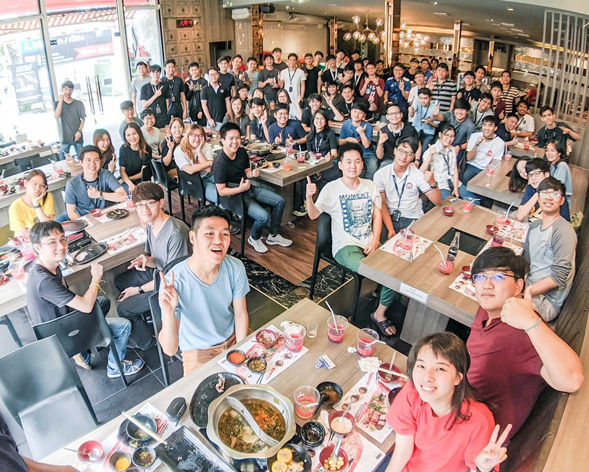
\includegraphics[width=0.47\textwidth]{eat}  
	}
	\subfigure[กิจกรรม WeShare]{
		\label{Fig:even1:weshare}
		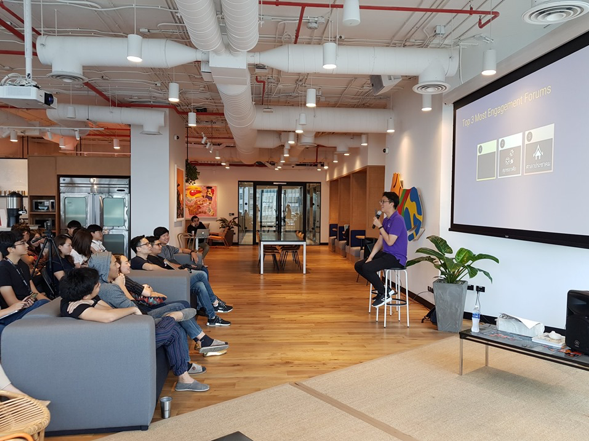
\includegraphics[width=0.4995\textwidth]{weshare}  
	}
	\subfigure[งาน Townhall]{
		\label{Fig:event1:townhall}
		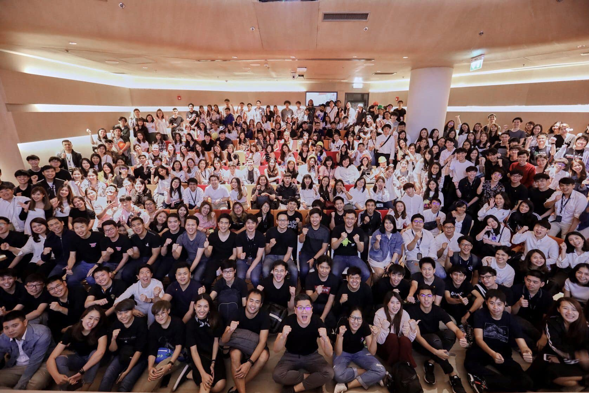
\includegraphics[width=1\textwidth]{townhall}  
	}
	\caption{กิจกรรมต่าง ๆ ระหว่างปฏิบัติงาน}
	\label{Fig:event1}
\end{figure}

ในช่วงท้ายของการปฏิบัติงานจะต้องมีการนำเสนอผลงานที่ได้ทำมาในช่วงปฏิบัติงาน ก็จะมีการจัดการซ้อมนำเสนอก่อนที่จะถึงวันนำเสนอจริง ๆ โดยจะต้องนำเสนอให้กับทีม Development ทั้งหมด และเป็นการนำเสนอแบบกลุ่ม โดยจะต้องนำเสนอร่วมกับนักศึกษาฝึกงานคนอื่นด้วย

\begin{figure}[!h]
	\centering
	\subfigure[การอบรมแนวทางการนำเสนอผลงาน]{
		\label{Fig:present:prepresent1}
		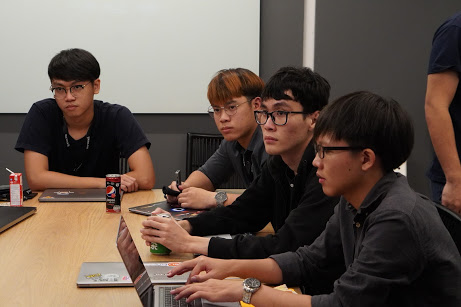
\includegraphics[width=0.475\textwidth]{prepresent1}  
	}
	\subfigure[การซ้อมนำเสนอผลงาน]{
		\label{Fig:present:prepresent2}
		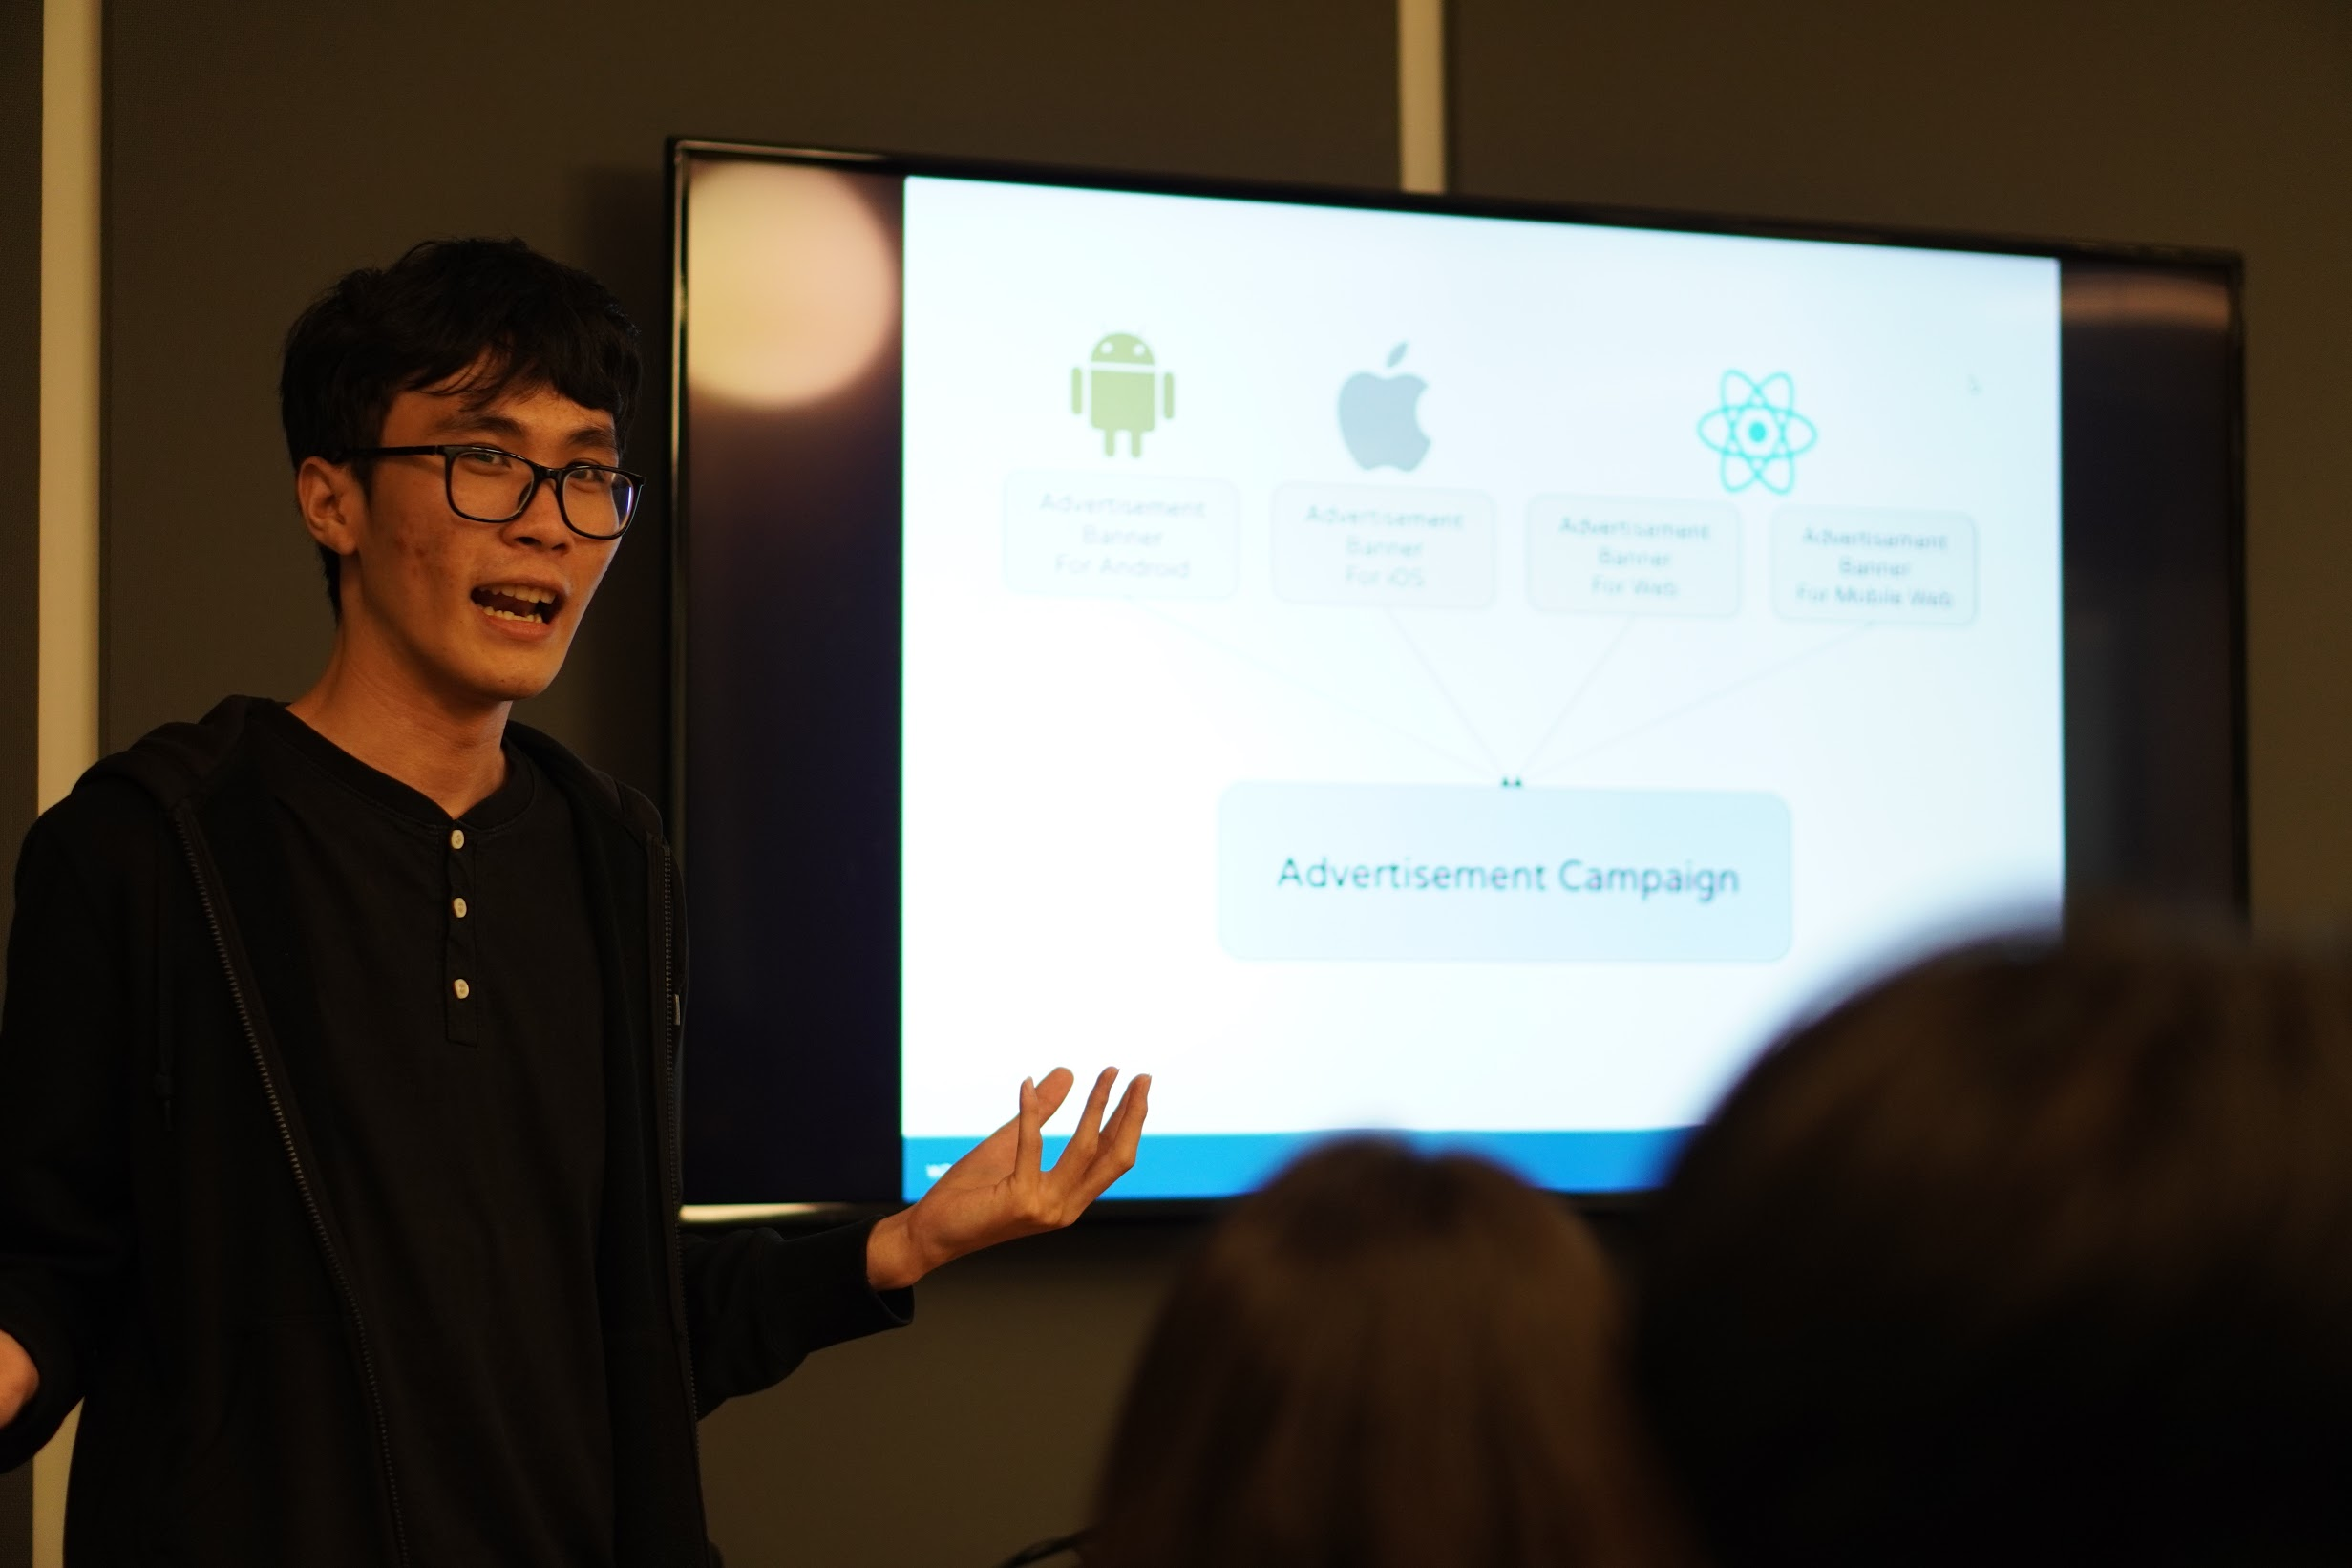
\includegraphics[width=0.475\textwidth]{prepresent2}  
	}
	\subfigure[การนำเสนอผลงานจริง]{
		\label{Fig:present:present1}
		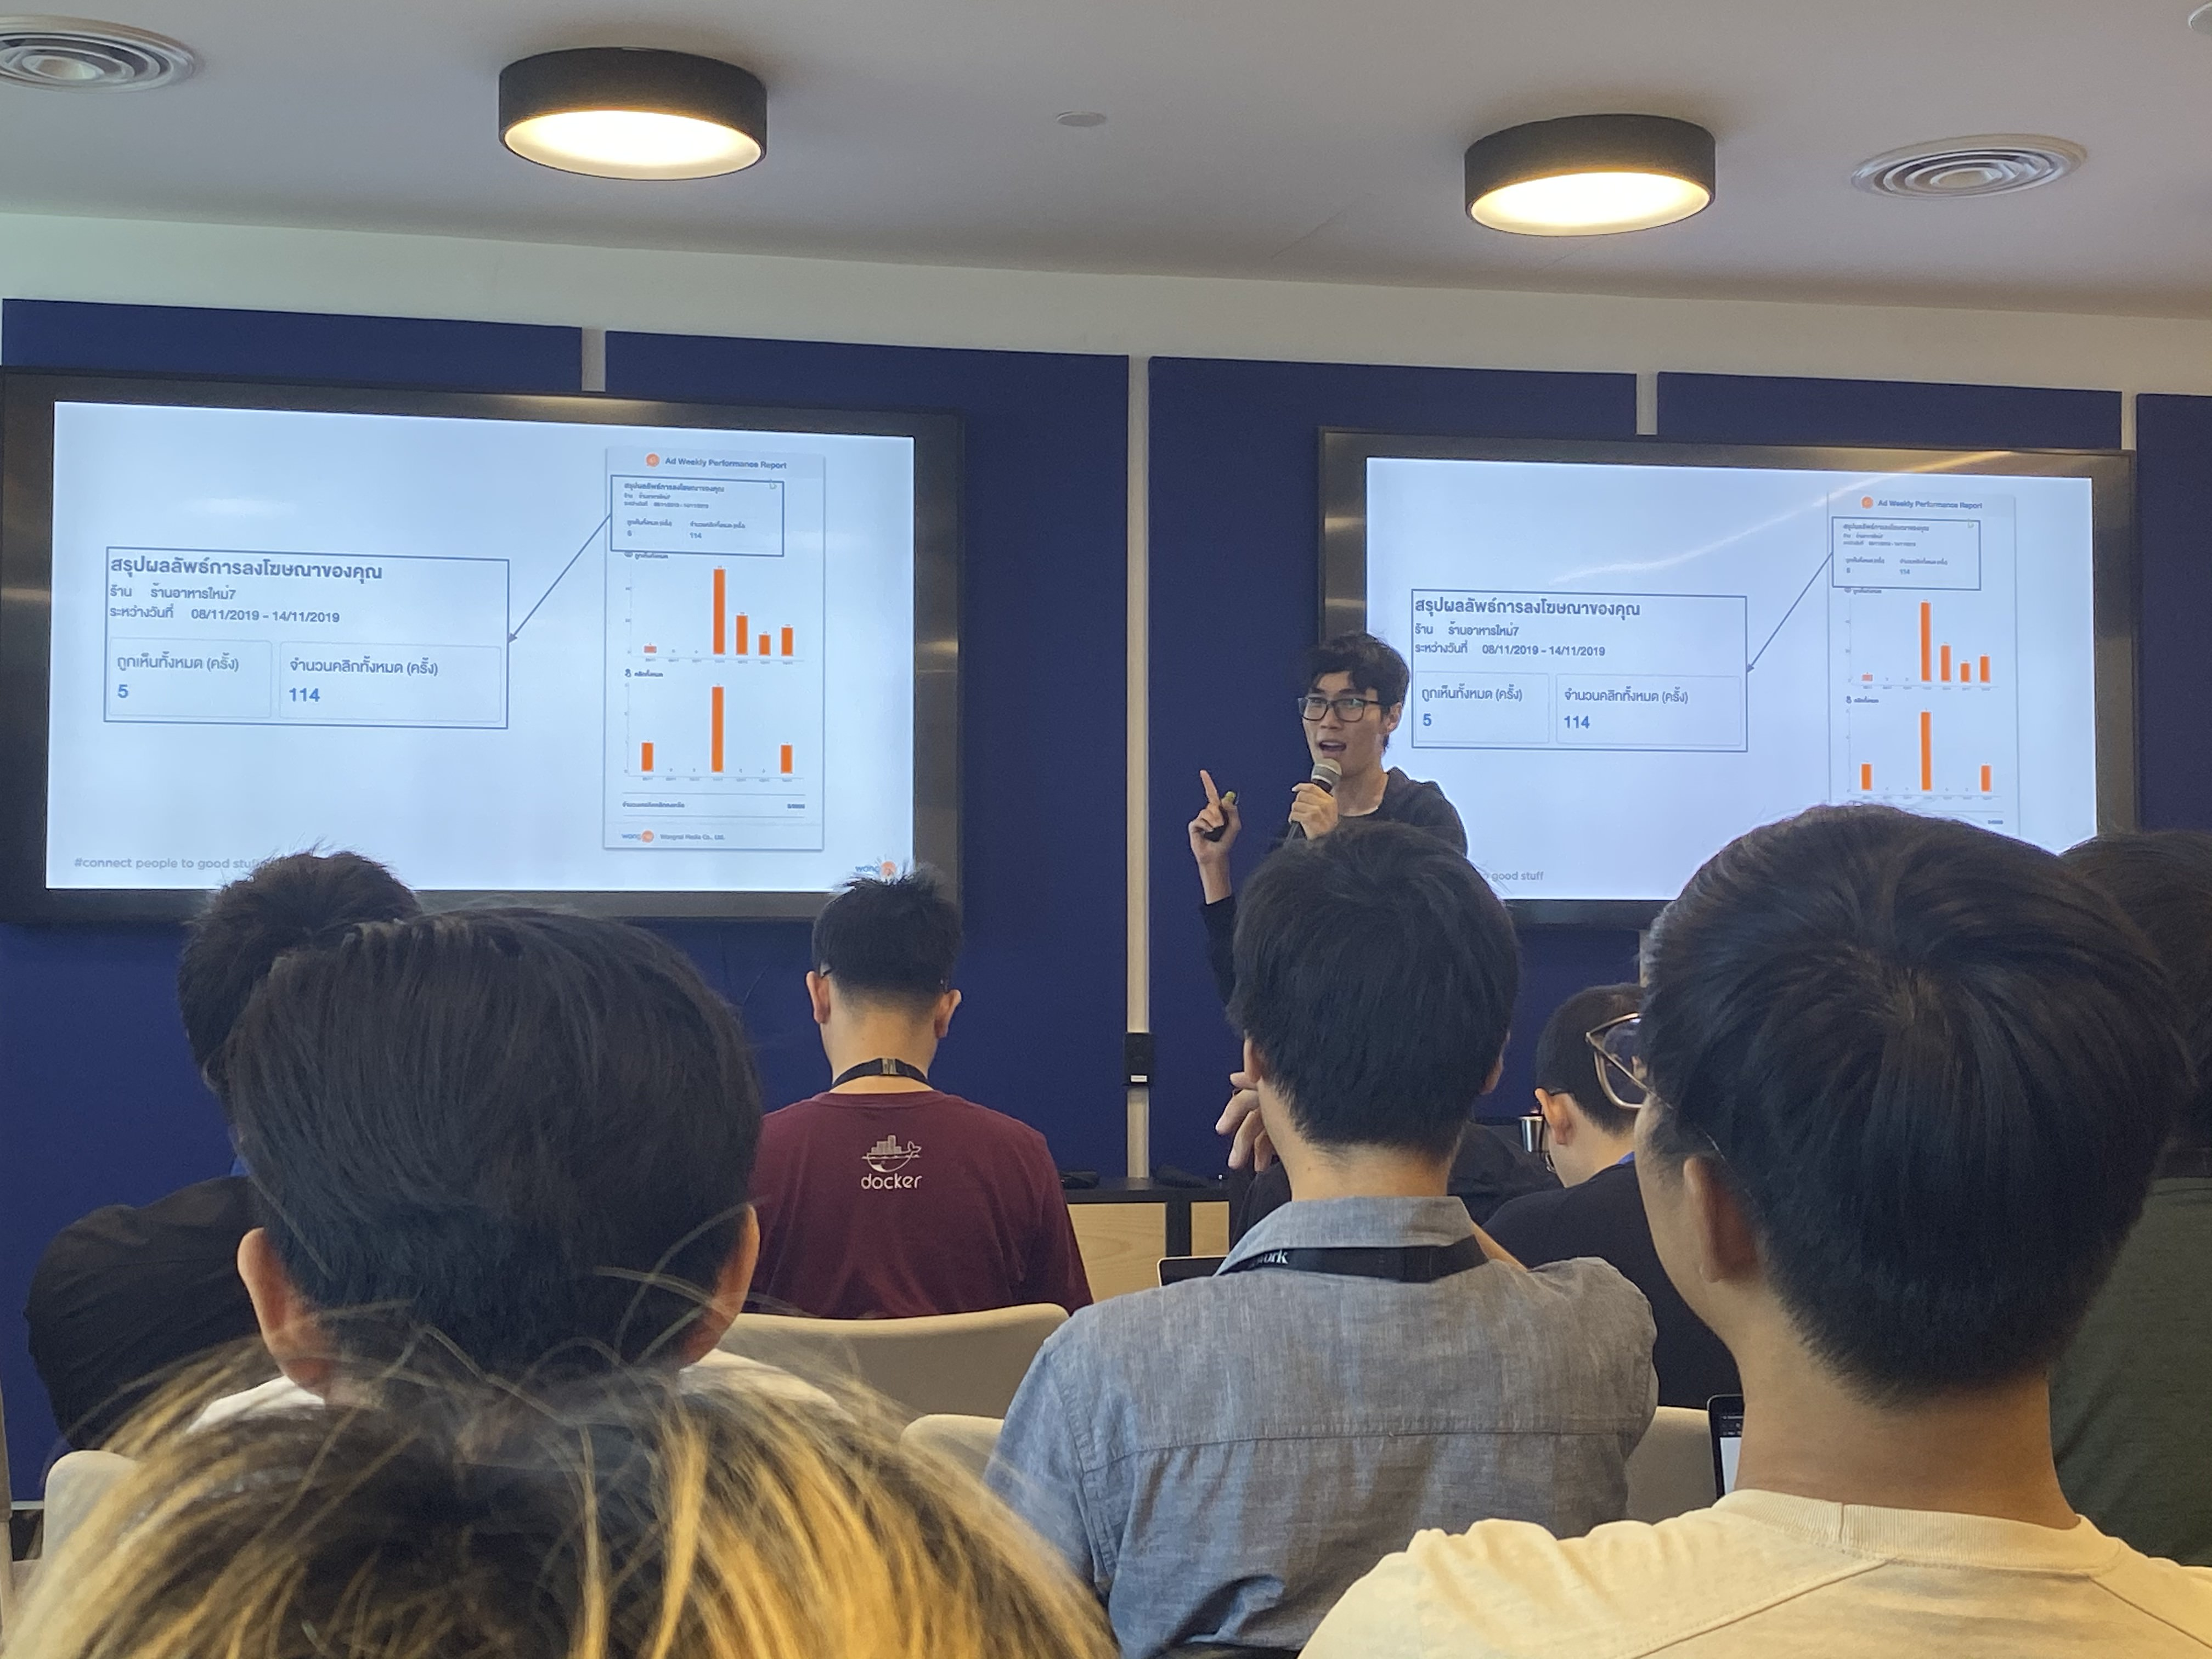
\includegraphics[width=0.475\textwidth]{present1}  
	}
	\subfigure[รูปรวมทีม Development หลังจากการนำเสนอผลงาน]{
		\label{Fig:present:present1}
		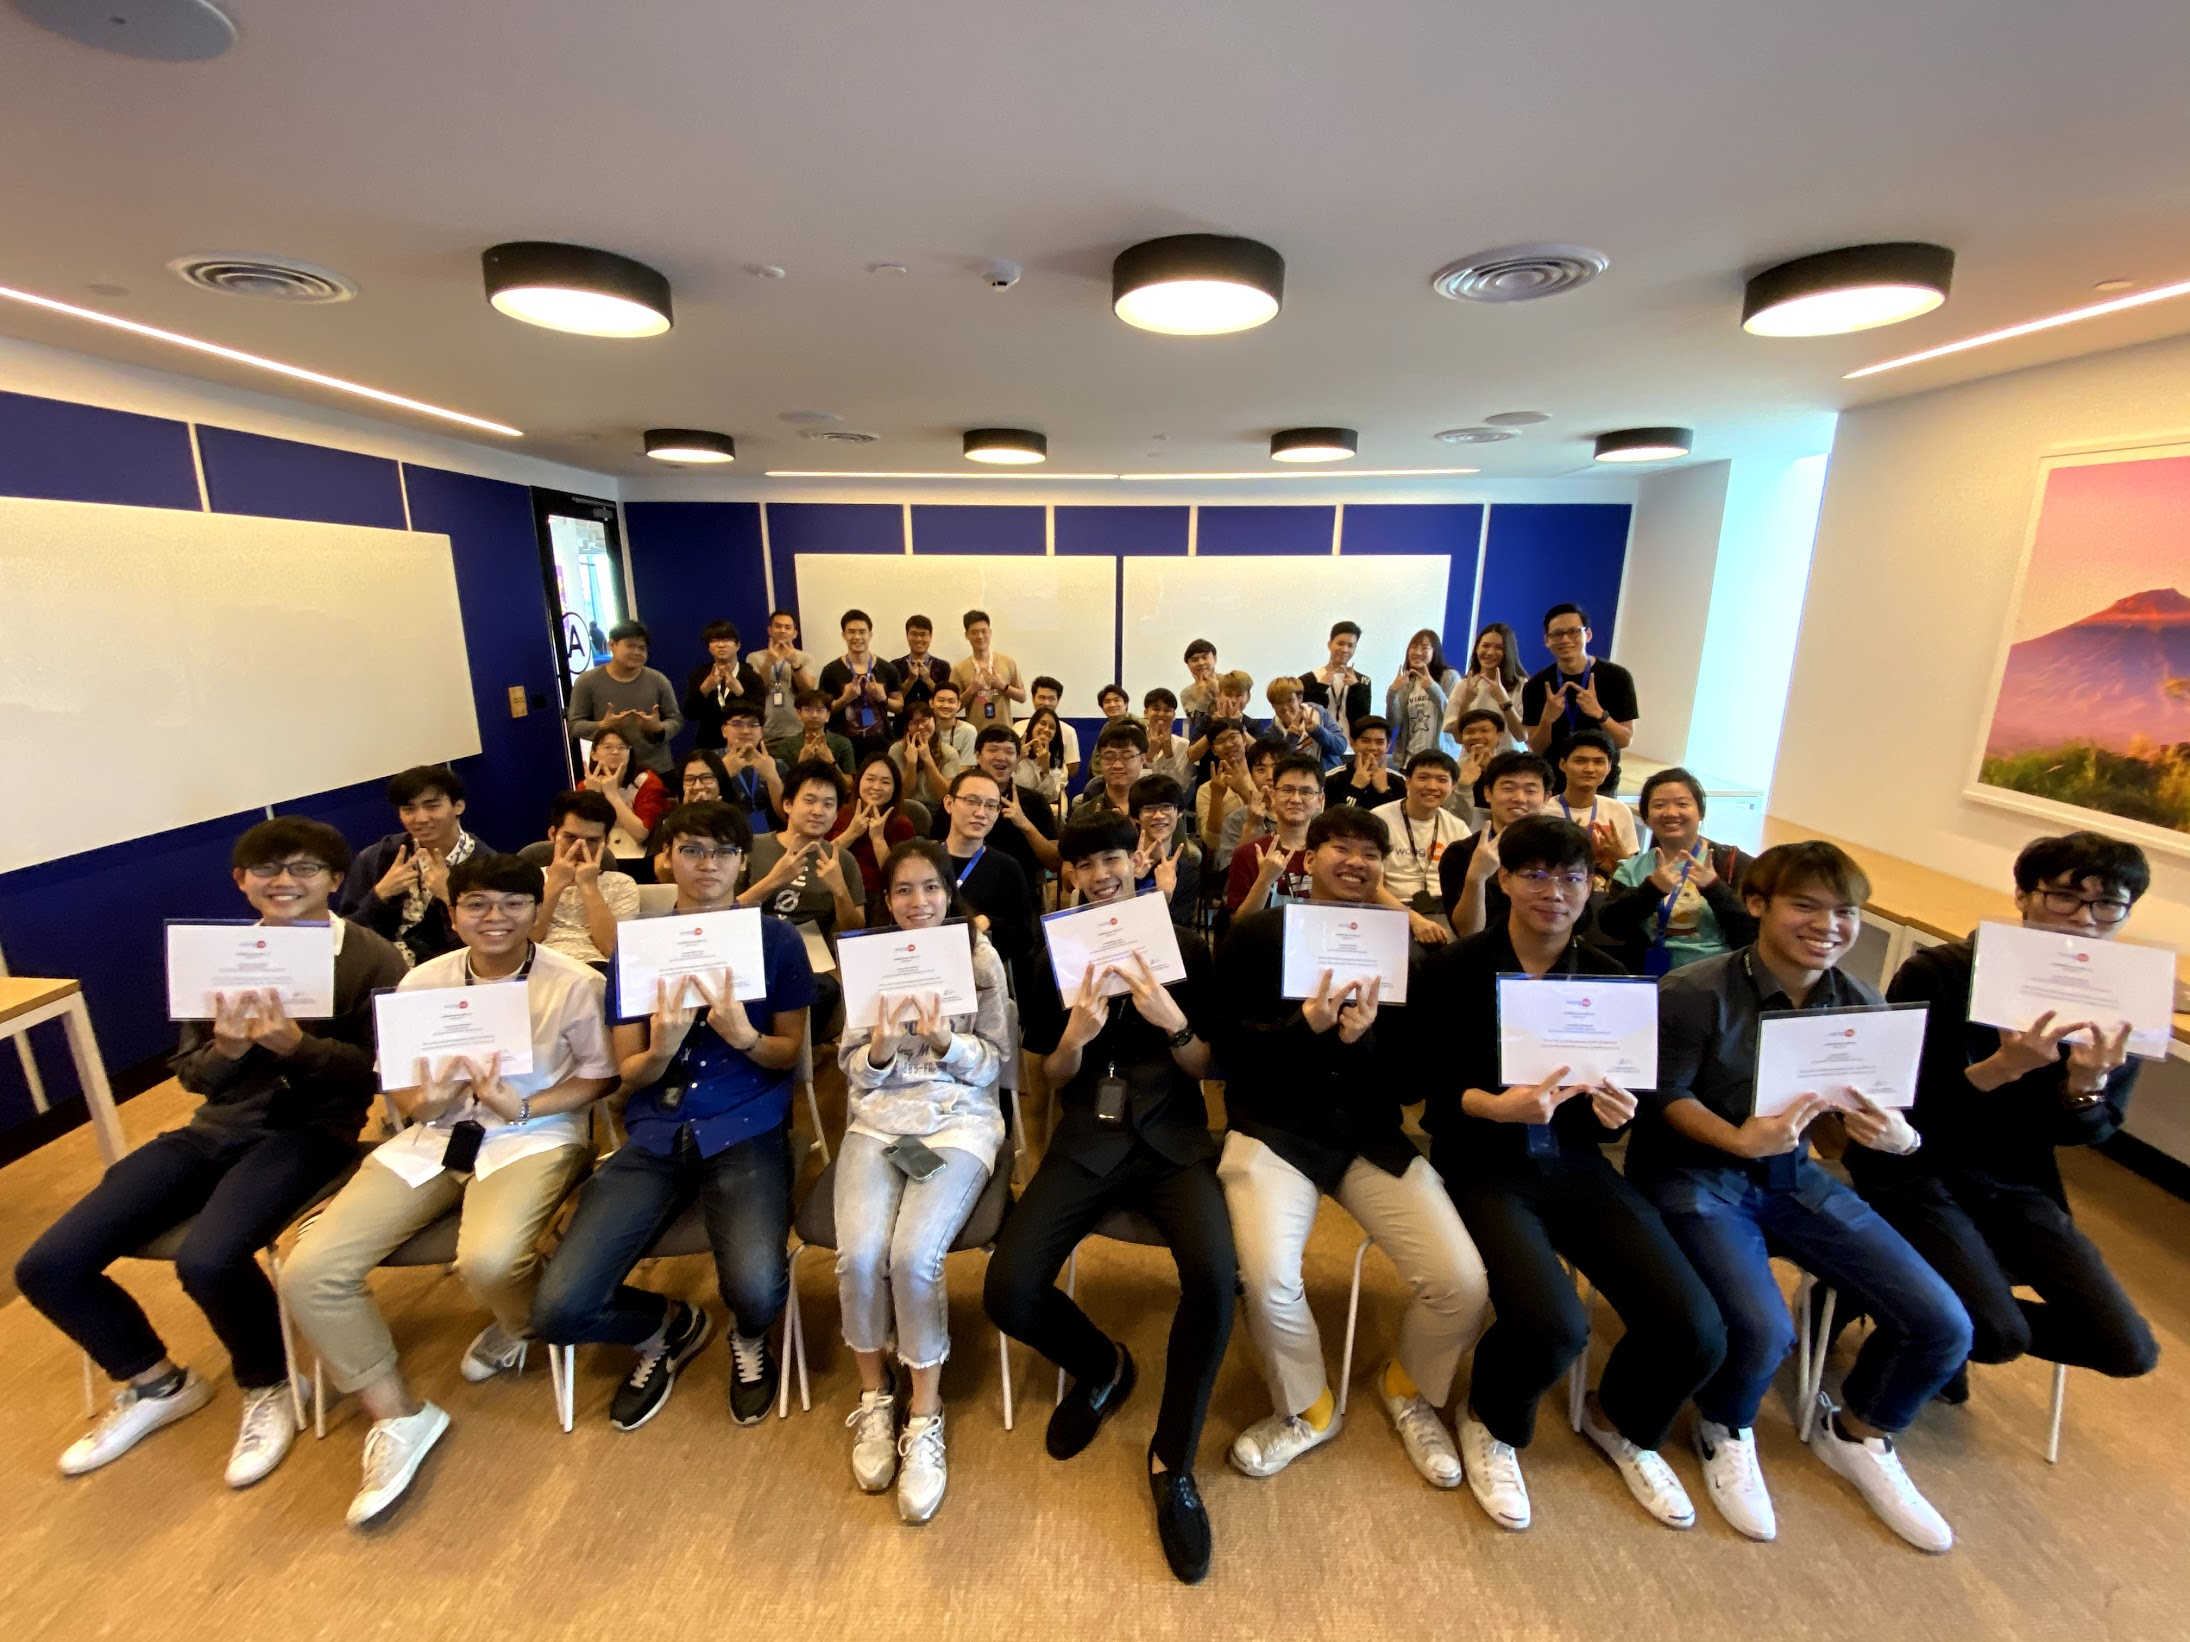
\includegraphics[width=0.475\textwidth]{present2}  
	}
	\caption{การซ้อมการนำเสนอผลงานและการนำเสนอผลงานจริง}
	\label{Fig:present}
\end{figure}

\chapter{ประวัติผู้เขียน}
\AddToShipoutPicture*
{\put(470,700){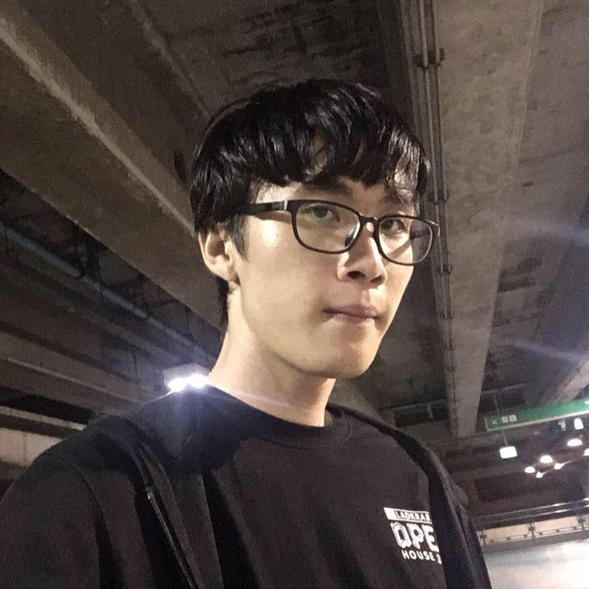
\includegraphics[width=3cm,height=3.1cm]{me.png}}}
\begin{tabularx}{\linewidth}{lX}
	\textbf{ชื่อ – นามสกุล} & มาวิน จงไกรรัตนกุล \\
	\textbf{Email} & mw.jkrtnk@gmail.com \\
	\textbf{ประวัติการศึกษา} & วิทยาศาสตร์​บัณฑิต สาขาวิชาเทคโนโลยีสารสนเทศ \\ & คณะเทคโนโลยีสารสนเทศ สถาบันพระจอมเกล้าเจ้าคุณทหารลาดกระบัง \\
\end{tabularx}